\documentclass[10pt,a4paper]{article}
\usepackage[utf8]{inputenc}
\usepackage[italian]{babel}
\usepackage{amsmath}
\usepackage{amsfonts}
\usepackage{amssymb}
\usepackage{graphicx}
\usepackage{gensymb}
\usepackage[left=2cm,right=2cm,top=2cm,bottom=2cm]{geometry}
\newcommand{\rem}[1]{[\emph{#1}]}

\author{Gruppo BN \\Lisa Bedini,  Federico Belliardo, Marco Costa}
\title{Esperienza 13: Semaforo}

\begin{document}
\maketitle

\section{Scopo dell'esperienza}
Lo scopo dell'esperienza è di realizzare un semaforo come macchina a stati finiti tale che
\begin{itemize}
\item nello stato ENABLED esegua un ciclo in cui si abbiano accesi (per la durata di un colpo di clock e nel seguente ordine) Led Verde, Led Verde e Giallo, Led Rosso.
\item nello stato NOT ENABLED faccia lampeggiare il Led Giallo (sincronamente  col clock).
\end{itemize}
Il semaforo è stato realizzato sia tramite circuiti integrati, sia programmando Arduino.

\section{Materiale a disposizione}
%correggi
\begin{itemize}
\item 2 SN7474 Dual D-FlipFlop
\item 1 SN7400 Quad NAND gate
\item 1 SN7408 Quad AND gate
\item 1 7432 Quad OR gate
\item DIP switch
\item 3 Led: verde, giallo, rosso
\end{itemize}
%I valori delle componenti sono state misurate con multimetro digitale (incertezza riportata sul manuale).
%Le differenze di potenziale sono state misurate tramite oscilloscopio, se non indicato diversamente, e come incertezza si è presa la sensibilità dei cursori più il 3\% di calibrazione.
%Per misurare i tempi si è usato l'oscilloscopio e come relativa incertezza si è preso il massimo fra la sensibilità dei cursori e la semidispersione dei valori plausibili.

\section{Stato Enabled}

Per realizzare il solo stato enabled abbiamo optato per una macchina di Moore, non essendoci alcun tipo di input. I tre stati della macchina sono 'Verde', 'Verde e Giallo', 'Rosso' (in una macchina di Moore le uscite sono determinate unicamente dallo stato). Abbiamo deciso di usare solo 2 FF in quanto due bit erano sufficienti per codificare i tre stati richiesti, poiché 'Verde' e 'Rosso' sono mutualmente esclusivi. Indicheremo sempre (anche nei punti successivi della relazione) $Q_1$ il bit più significativo, mentre $Q_0$ sarà sempre il bit meno significativo della codifica. In figura \ref{fig:FSMenabled} abbiamo disegnato le transizioni, la codifica in bit dei vari stati e relative uscite.
\begin{figure}[!htb]
\centering
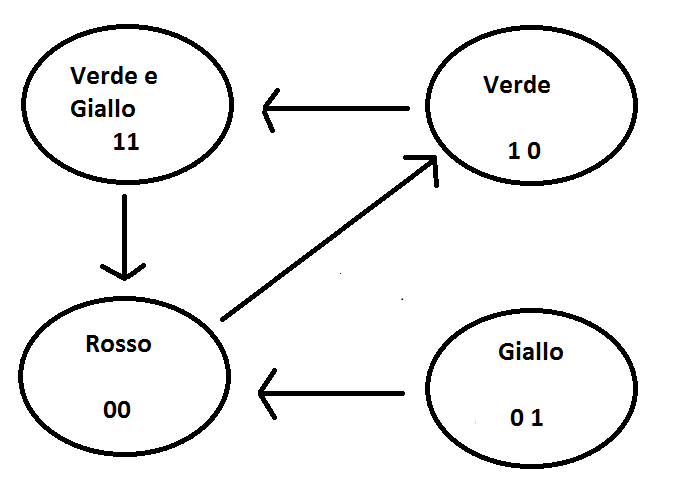
\includegraphics[scale=0.7]{FSMenabled.png}
\caption{Diagramma dello stato Enabled. Le transizioni avvengono ad ogni colpo di clock.\label{fig:FSMenabled}}
\end{figure}
%In arrivo frase ambigua
Abbiamo deciso di codificare lo stato logico rimanente ($Q_1 = 0$, $Q_0 = 1$ in termini di bit) come lo stato fisico in cui il solo Led Giallo è acceso. Tale stato compare nel circuito solo nella eventualità in cui i FF si accendano in questa configurazione. Salvo in questo caso, 01 non compare più nei cicli successivi.
Il vantaggio di questa codifica è che il Led Verde e il Led Giallo sono pilotati da due bit distinti, rispettivamente $Q_1$ e $Q_0$ nel nostro caso. In questo modo ci sarà più facile in seguito poter far lampeggiare il solo Led Giallo.
Le tabelle di transizione implementate sono riportate in tabella \ref{tab:transizioneenabled}. I \emph{don't care} sono già stati assegnati in questa tabella. Nelle sezioni successive daremo una breve spiegazione su come sono stati eliminati. Nella tabella $D_0$ e $D_1$ rappresentano gli ingressi dei Flip-Flop. Come si può vedere dalla tabella le uscite $Q_{1,n+1}$ e $Q_{0,n+1}$ diventano gli ingressi dei FF $D_{1, n}$ e $D_{0, n}$.

%TODO Forse non è più esatto scrivere D_{n+1}

\begin{table}[!htb]
\centering
\begin{tabular}{|c|c|c|c||c|c||c|c|c|}
\hline
$Q_{1,n}$ & $Q_{0,n}$ & $D_{1, n}$ & $D_{0, n}$& $Q_{1,n+1}$ & $Q_{0,n+1}$ & $LV$ & $LG$ & $LR$\\
\hline
0 & 0 & 1 & 0 & 1 & 0 & 0 & 0 & 1 \\
0 & 1 & 0 & 0 & 0 & 0 & 0 & 1 & 0\\
1 & 0 & 1 & 1 & 1 & 1 & 1 & 0 & 0\\
1 & 1 & 0 & 0 & 0 & 0 & 1 & 1 & 0\\
\hline
\end{tabular}
\caption{Tabella di verità delle transizioni fra stato $n$ e il successivo $n+1$, e delle uscite (in funzione dello stato $n$).\label{tab:transizioneenabled}}
\end{table}
\subsection{Funzioni logiche delle transizioni}
Nella funzione di transizione, abbiamo libertà di scegliere la transizione dello stato 'Giallo' 01.
Con una semplificazione tramite mappe di Karnaugh si ottiene che ponendo i due \emph{don't care} 
\footnote{In realtà non sono propriamente dei \emph{don't care}: è' lecito assegnare a questi  tutte le combinazione tranne 01, caso in cui la macchina resterebbe perpetuamente in questo stato.} pari a 0 si ottiene che la funzione logica richiesta è \begin{equation}
Q_{1, n+1} = \bar {Q}_{0,n} \qquad Q_{0,n+1} = \bar {Q}_{0,n} \cdot Q_{1,n} 
\end{equation}
Così si ha che lo stato non richiesto 01 ("solo giallo acceso"), transisce nello stato 00 ("solo rosso acceso").
%TODO Se ho capito bene la frase direi che è totalmente inutile.
Dato che abbiamo dei FF di tipo D, il valore di $Q_{i, n+1}$ è uguale al valore dell'ingresso $D_i$ nello stato $n$: minimizzare quindi il numero di operazioni logiche nelle funzioni dei $Q_{i,n+1}$ effettivamente minimizza il numero di porte logiche da implementare fisicamente.

\subsection{Funzioni logiche delle uscite}
Una volta codificati gli stati, abbiamo assegnato alle uscite $LV$ (Led Verde), $LG$ (Led Giallo), $LR$ (Led Rosso) i seguenti valori:
\begin{equation}
LV = Q_1 \qquad LG = Q_0 \qquad LR = \bar{Q}_0\cdot \bar{Q}_1
\end{equation}
Questo era in effetti il modo più semplice per realizzare i collegamenti fra i FF e le uscite: per come sono stati codificati gli stati, i Led Verde e Giallo sono pilotabili direttamente dal rispettivo bit, mentre per il Led Rosso abbiamo scelto l'unica funzione che valga 1 solo sullo stato 00. 

%In effetti avremmo pure potuto prendere come funzione per pilotare il Led rosso $\bar{Q_1}$, a patto però di avere 01 stato in cui sia il giallo che il rosso sono accesi. Abbiamo preferito usare una porta in più qui e avere la possibilità di controllare il Led giallo direttamente.
%TODO: non ho capito a cosa di rifersci on la riga sotto... XD Era un commento stupido circa la parte virgolettata sopra, che è inutile e infatti è commentata
%non mi piace come è scritta questa parte: ad esempio all'inizio dico subito che lo stato 0 1 è il giallo ma solo ora dichiao in effetti a cosa sia collegata l'uscita L_G... Inoltre, sebbne la tabella di transizione la ho scritta bene, devo far capire che poi i q_n+1 sarebbero gli ingressi D...
\subsection{Implementazione del circuito}
Abbiamo implementato il circuito come in figura \ref{fig:circenable}.
\begin{figure}[!htb]
\centering
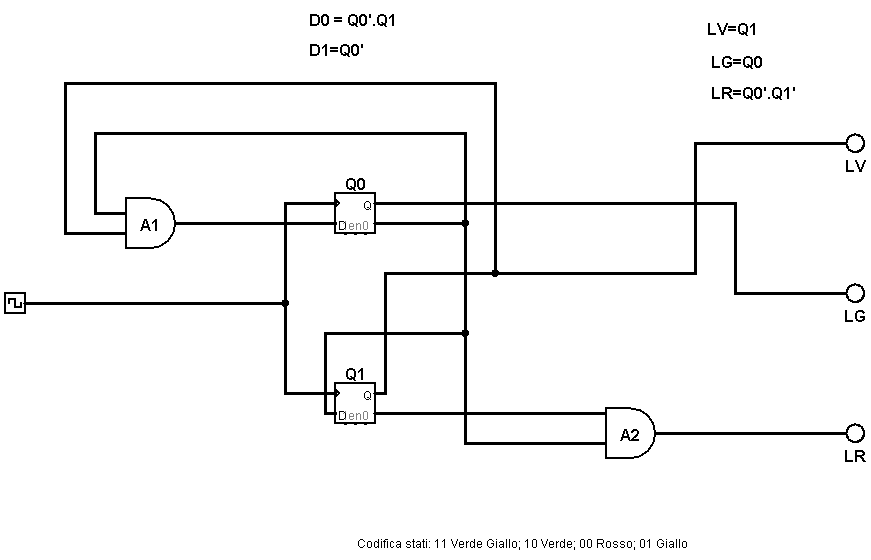
\includegraphics[scale=0.5]{circenable.png}
\caption{Circuito implementato per il solo stato Enabled. Nella figura non si sono riportati per semplicità i collegamenti dei LED a terra , le alimentazioni e i collegamenti dei Preset e Clear. $E$ è collegato a massa tramite interruttore: se è aperto vale 1 (logica TTL), se chiuso 0\label{fig:circenable}}
\end{figure}
Sono stati collegati i Clear e Preset dei FF alla tensione di alimentazione $V_{CC} = 4.9\pm0.1 $V\footnote{Misurata tramite multimetro digitale; incertezza riportata sul manuale} tramite resistenze di pull-up di valore nominale di $1.5\,\mbox{k}\Omega$. Abbiamo collegato i Led a terra tramite resistenze da $330\,\Omega$ nominali che hanno lo scopo di limitare la corrente.
Le forme d'onda del clock e del segnale a ciascuno dei tre Led sono state acquisite mediante l'oscilloscopio.

\begin{figure}[!htb]
\centering
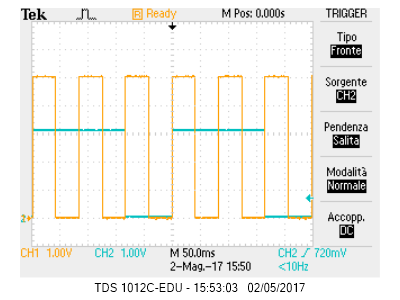
\includegraphics[scale=0.7]{clock-verde.png}
\caption{In CH1 il segnale del clock, in CH2 quello del Led Verde.\label{fig:verde}}
\end{figure}

\begin{figure}[!htb]
\centering
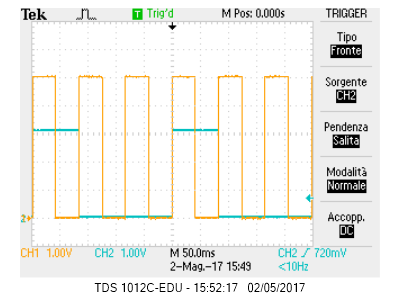
\includegraphics[scale=0.7]{clock-gialloverde.png}
\caption{In CH1 il segnale del clock, in CH2 quello del Led Giallo.\label{fig:giallo}}
\end{figure}

\begin{figure}[!htb]
\centering
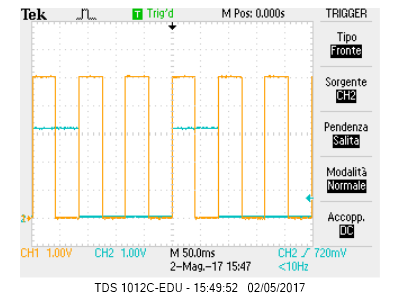
\includegraphics[scale=0.7]{clock-rosso.png}
\caption{In CH1 il segnale del clock, in CH2 quello del Led Rosso.\label{fig:rosso}}
\end{figure}

Si osservi che i segnali dei Led (e quindi delle uscite dei FF, a meno di ritardi trascurabili) diventano positivi quando il clock è sul fronte positivo (abbiamo utilizzato dei \emph{positive-edge triggered} Flip-Flop). Inoltre, come atteso, si osserva che il Led Giallo e Rosso stanno accesi per un periodo di clock e spenti per i due successivi (Figure \ref{fig:giallo} e \ref{fig:rosso}), mentre il Verde si comporta al contrario cioè sta acceso per due periodi e spento per il successivo (Figura \ref{fig:verde}).

\section{Semaforo completo}
Abbiamo scelto di usare una macchina di Mealy per realizzare il semaforo completo. Si è mantenuta la stessa codifica degli stati in termini di bit utilizzata precedentemente. In questo modo la funzione di transizione nello state Enabled è identica a quella precedente. Abbiamo chiamato E il valore logico dell'enable.
%TODO spiega meglio perchè per convenianza si è scelto quello. Così ti garba?
Si è deciso (per convenienza) di scegliere lo stato Enabled quando $E = 1$ (e attivo alto): in questo modo possiamo disabilitare una uscita nello stato Not Enabled semplicemente con una porta AND fra l'uscita e $E$. In tabella \ref{tab:semaforocompleto} abbiamo riportato le transizioni dei FF (i \emph{don't care} sono già stati assegnati), mentre in figura \ref{fig:FSMcomplete} è stata disegnata la mappa schematica delle transizioni (nella figura gli output sono stati codificati nell'ordine LV-LG-LR).

\begin{figure}[!htb]
\centering
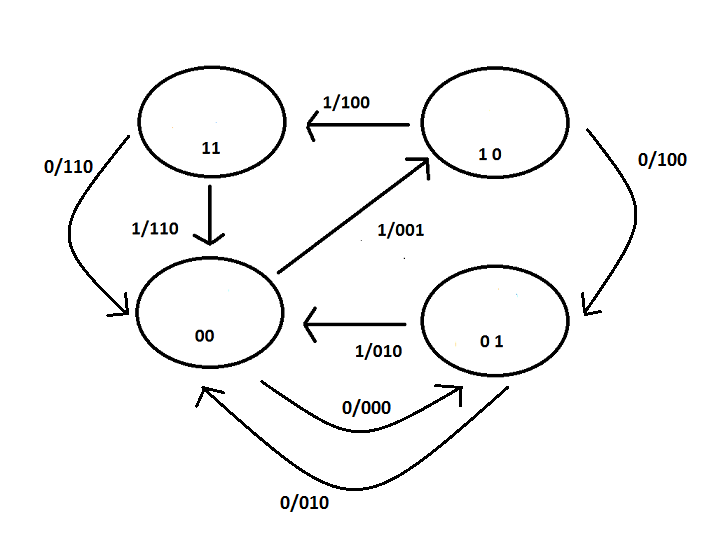
\includegraphics[scale=0.7]{FSMcomplete.png}
\caption{Diagramma delle transizioni per la macchina di Mealy realizzata. La terna degli output è LV-LG-LR.\label{fig:FSMcomplete}}
\end{figure}


\begin{table}
\centering
\begin{tabular}{|c||c|c|c|c||c|c||c|c|c|}
\hline
$E$ & $Q_{1,n}$ & $Q_{0, n}$ & $D_{1,n}$ & $D_{0,n}$ & $Q_{1, n+1}$ & $Q_{0, n+1}$ & $LV$ & $LG$ & $LR$\\
\hline
0 & 0 & 0 & 0 & 1 & 0 & 1 & 0 & 0 & 0 \\
0 & 0 & 1 & 0 & 0 & 0 & 0 & 0 & 1 & 0\\
0 & 1 & 0 & 0 & 1 & 0 & 1 & 1 & 0 & 0\\
0 & 1 & 1 & 0 & 0 & 0 & 0 & 1 & 1 & 0\\
\hline
1 & 0 & 0 & 1 & 0 & 1 & 0 & 0 & 0 & 1 \\
1 & 0 & 1 & 0 & 0 & 0 & 0 & 0 & 1 & 0\\
1 & 1 & 0 & 1 & 1 & 1 & 1 & 1 & 0 & 0\\
1 & 1 & 1 & 0 & 0 & 0 & 0 & 1 & 1 & 0\\
\hline
\end{tabular}
\caption{Matrice di transizione e valori di verità per le uscite nel caso di semaforo completo. (Uscite funzione dello stato $n$). \label{tab:semaforocompleto}}
\end{table} 


\subsection{Funzioni logiche delle transizioni}
%TODO Di con esattezza tra cosa e cosa è l'AND che ti permette di tenere il circuito precedente. Così ti piace?
Nel caso Not Enabled, abbiamo deciso di mantenere lo stato logico 01 come stato fisico con solo il Led Giallo acceso. Si è deciso (arbitrariamente) di farlo transire verso 00 (che sarà lo stato con uscite tutte spente). Infatti in modalità Enabled lo stato 00 ha solo il Led Rosso acceso, pertanto con l'aggiunta di un AND fra questo ed il bit E si è riusciti ad avere tutte le uscite spente, mantenendo il circuito costruito in precedenza. Le transizioni degli altri stati (10 e 11) sono state scelte in modo che le relative mappe di Karnaugh risultassero le più semplici possibili compatibilmente col fatto che gli stati 10 e 11 non devono ricomparire più nel ciclo.
Abbiamo così ottenuto come funzioni logiche per le transizioni:
\begin{equation}
Q_{0, n+1} = \bar{Q}_{0,n}\cdot(\bar{E}+Q_{1,n})\qquad
Q_{1, n+1} = E\cdot \bar{Q}_{0, n}
\end{equation}
\subsection{Funzioni logiche delle uscite}
Con lo stesso modo si sono scelte le funzioni di output dei Led relativamente ai soliti stati indesiderati 11 e 10. Stavolta i valori logici degli output sono dei veri \emph{don't care} (possiamo effettivamente assegnare ad essi qualsiasi valore logico). Si sono scelte dunque le seguenti equazioni:
\begin{equation}
LV = Q_1\qquad LG = Q_0\qquad LR = E\cdot(\bar{Q}_1\cdot\bar{Q}_0)
\end{equation}
Si osservi che il Led Verde in teoria può essere acceso nello stato Not Enabled, ma questo può accadere solo se la macchina viene inizializzata in uno degli stati in cui è acceso. Dopo il primo colpo di clock il Led Verde si spegne e non si riaccende più. La macchina entra infatti nell'oscillazione desiderata.\\

\subsection{Implementazione del circuito}
Abbiamo implementato il circuito in figura \ref{fig:circcomplete}.
\begin{figure}[!htb]
\centering
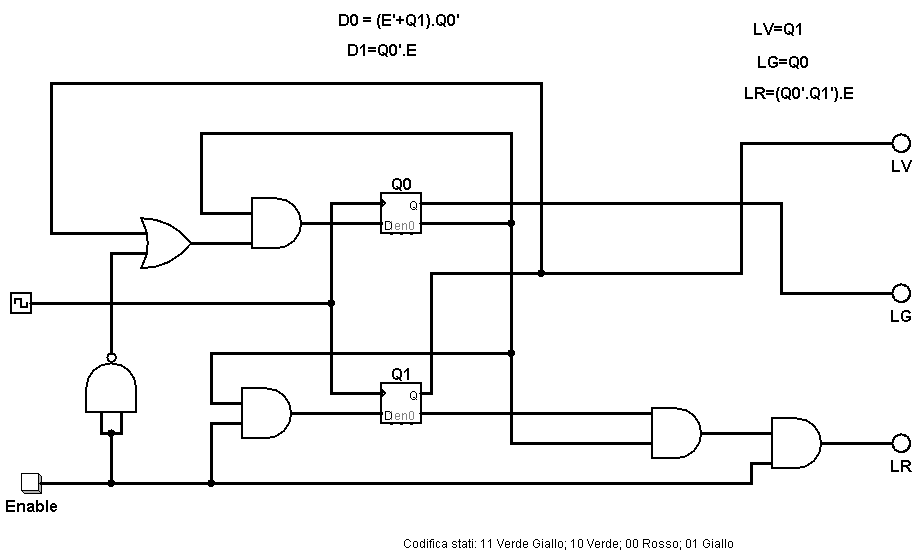
\includegraphics[scale=0.5]{circcomplete.png}
\caption{Circuito implementato con Enable. Nella figura non si sono riportati per semplicità i collegamenti dei LED a terra , le alimentazioni e i collegamenti dei Preset e Clear. $E$ è collegato a massa tramite switch: se è aperto vale 1 (logica TTL), se chiuso 0\label{fig:circcomplete}}
\end{figure}
%figura circuito con piedini numerati
Si osservi che in questa situazione è stato implementato un meccanismo di abilitazione asincrona: non appena si cambia lo stato di $E$, indipendentemente dal fronte del clock, si ha che i Led cambiano stato con effetto immediato. Dalla figura \ref{fig:circcomplete} si può in effetti vedere che il passaggio di $E$ da 1 a 0 disabilita istantaneamente la porta AND A3 che precede il Led Rosso. Si osservi tuttavia che lo stato dei FF non è cambiato: questi cambiano solo dopo un colpo di clock. Dunque in un certo senso l'effetto dell'abilitazione asincrona del semaforo rende indefinito lo stato del semaforo fino al prossimo colpo di clock.\\
In figura \ref{fig:lampeggiante} possiamo osservare come nello stato Not Enabled il Led Giallo si accenda e si spenga il periodo di clock successivo. Il semaforo funziona come programmato.

\begin{figure}
\centering
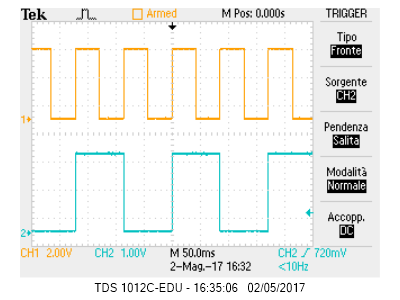
\includegraphics[scale=0.7]{ch1clock-ch2giallolamp.png}
\caption{In alto il sengale del clock, in basso l'uscita al Led Giallo in modalità Not Enabled.\label{fig:lampeggiante}}
\end{figure} 

%Il Led Rosso è collegato all'enable non tramite altri D-Latch, quindi  se è acceso mentre $E$ passa da 1 a 0, avviene immediatamente il cambio dei valori logici delle uscite previste nel caso di $E = 0$, ossia si passa all'uscita $LG=1$ senza aspettare il clock.
%Per le altre uscite non ci sono problemi in quanto sono collegate ad $E$ solo tramite i vecchi D-Latch.

\subsection{Abilitazione sincrona}
Per realizzare un meccanismo di abilitazione sincrona, ossia per fare in modo che il semaforo registri solo cambiamenti di $E$ che avvengono sul fronte alto del clock, si è collegato $E$ all'AND A3 (che causava cambi di output istantanei) tramite un terzo D-Latch, come in figura \ref{fig:circcompletesincrono}.
E' sufficiente l'aggiunta di questo solo FF perché gli altri due collegamenti che coinvolgono l'Enable sono verso gli ingressi D dei FF, che registrano i cambiamenti degli input in modo sincrono.
\begin{figure}[!htb]
\centering
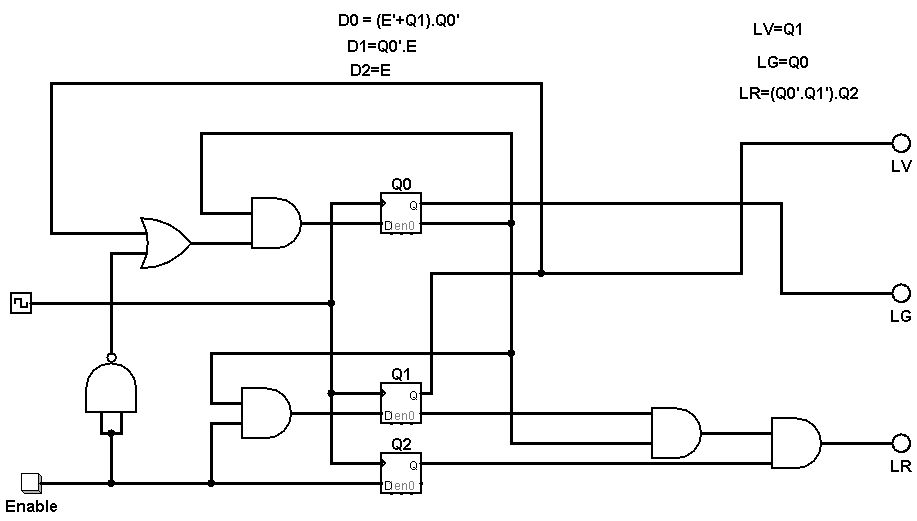
\includegraphics[scale=0.5]{circcompletesincrono.png}
\caption{Circuito implementato con abilitzione sincrona. Nella figura non si sono riportati per semplicità i collegamenti dei LED a terra , le alimentazioni e i collegamenti dei Preset e Clear. $E$ è collegato a massa tramite interruttore: se è aperto vale 1 (logica TTL), se chiuso 0\label{fig:circcompletesincrono}}
\end{figure}

%TODO Nella relazione hai gi scritto che implementi quello che non passa per il VERDE?
%Sì, questo circuito non passa per il VERDE
%Si osservi che a differenza di prima, si osserva una transizione diversa se passiamo da Enabled a Not Enabled quando ci troviamo nello stato 00 (Led Rosso acceso); nel circuito costruito prima si passa subito a stato spento 00, che poi transisce a 01 (ossia con il solo Led Giallo acceso). Adesso si ha una transizione a 10, in cui si ha il Led Verde acceso, e poi si entra nel ciclo 00/01, in cui si ha il Led Giallo lampeggiante.

\section{Semaforo con Arduino}
Adesso vogliamo implementare lo stesso semaforo programmando Arduino. Abbiamo optato per una macchina di tipo Moore, più semplice concettualmente da realizzare.
Abbiamo collegato le uscite di Arduino 9, 10, 11 tramite il buffer rispettivamente ai Led Verde, Giallo, Rosso, inserendo resistenza da $330\Omega$ su ciascuno per limitare la corrente.
Queste uscite sono state dichiarate come OUTPUT nel programma utilizzato.
L'enable è stato collegato all'uscita 8, e nel programma è dichiarato come INPUT-PULLUP (ossia alto se interruttore aperto e basso se chiuso).
Su Arduino ad ogni Led è stato assegnato un bit, la codifica è quindi quella banale. Sono stati considerati solo i vari stati che ci servono: quelli indesiderati non si presentano mai dato che l'inizializzazione (nello stato in cui tutto è spento) viene fatta da noi nel programma (all'interno dell'\emph{init}) e non casualmente come nel caso dei FF.
Il funzionamento del programma mima il comportamento della macchina a stati finiti precedentemente costruita:
\begin{itemize}
\item Legge il valore dell'Enable (attivo alto)
\item Legge lo stato in cui si trova attualmente
\item Calcola lo stato successivo in cui andare a seconda dello stato attuale e del valore di Enable
\item Accende i Led relativi allo stato in cui si trova la macchina (è di tipo Moore, quindi lo stato determina le uscite) e attende per il tempo preimpostato.
\item Dopo l'attesa, ripete il ciclo dall'inizio
\end{itemize}
Si osservi che in questa macchina si ha una abilitazione sincrona (avviene solo ad inizio ciclo la lettura dell'input).
Il programama utilizzato è stato preso dalla documentazione di Arduino del sito di LAB3; si è provato ad eseguire qualche semplice modifica (tempo permanenza in ciascuno stato, diversi stati di uscita) ma lo scheletro è sempre rimasto quello descritto sopra.
\section{Conclusioni}
Abbiamo concluso con successo le realizzazioni delle macchine secondo le specifiche richieste. Si è realizzato in aggiunta un meccanismo di Enable sia asincrono che sincrono per il semaforo costruito con i FF.
\end{document}







